\subsection{The Orbit and the Message: From Kepler to Control}

Take \textbf{Kepler’s Second Law}: a planet sweeps out equal areas in equal times as it orbits the Sun. At first glance, it seems like a geometric curiosity—a simple regularity traced from the meticulous observations of Tycho Brahe and Kepler’s inspired interpretation. It’s often celebrated as a triumph of empiricism: celestial mechanics revealed through patient data and careful curve-fitting.

But Kepler’s law holds more than geometry—it carries structure, constraint, and a whisper of optimization. Beneath the symmetry lies a principle of motion: conservation of angular momentum. Newton formalized this in terms of force and mass. A planet, acted on by gravity alone, experiences no torque about the Sun, so its angular momentum remains unchanged. Equal areas in equal times is the visible shadow of that invisible constancy.

From the classical viewpoint, this is cause and effect: torque-free motion under a central force gives rise to geometric regularity.

But \textbf{control theory} tells a different story.

In Pontryagin’s Maximum Principle (PMP), a physical system evolves in time as the solution to an optimal control problem—one that minimizes or maximizes some functional. Even if there are no explicit control inputs, the system behaves as though it were making strategic choices to follow a path of minimal cost or maximal structure.

And here’s where it gets interesting.

In this formulation, every state variable (like angular position \( \theta \)) has a \textbf{costate}—a kind of dual variable, or dynamic “price tag,” that tracks how sensitive the system's performance is to changes in that state.

For the orbiting planet, the costate \( \lambda_\theta \) associated with \( \theta \) turns out to be:
\[
\lambda_\theta = \frac{\partial H}{\partial \dot{\theta}} = L
\]
That’s angular momentum.

So while Newton described angular momentum as a conserved quantity due to a lack of torque, Pontryagin sees it as something deeper: a sensitivity measure, tracking how “valuable” it is to change \( \theta \). The planet doesn’t choose where to go—but its structure acts as if it’s preserving something essential.

This reframes Kepler’s Second Law in dynamic terms. It’s not just a geometric artifact—it’s a condition that must hold for the system’s path to remain optimal.

\begin{quote}
\textbf{The orbit is a solution. Not to a force equation, but to a structural question:}  
How can motion unfold while preserving the value attached to a particular change?
\end{quote}

This shift in perspective marks more than a mathematical reinterpretation—it reflects a philosophical one. Kepler described nature’s patterns. Newton gave them causes. Pontryagin suggests that even passive systems obey a logic of evaluation—where movement is shaped not just by force, but by the sensitivity of outcomes to the states they pass through.

In this view, \textbf{the costate is the silent guide}. It doesn't push or pull. It whispers:  
\textit{“Here is what matters. Preserve it.”}

\begin{tcolorbox}[colback=blue!5!white, colframe=blue!50!black,
title={Sidebar: What the Costate Really Means}]
The costate \( \lambda \) is the unsung character in optimal control—a mathematical shadow that tells us:

\begin{itemize}
  \item How much impact a small change in state has on the system’s future behavior.
  \item What value the system implicitly assigns to being “here” vs. being “there.”
  \item Which paths preserve what matters—even in systems without choices.
\end{itemize}

In our planetary case:
\[
\lambda_\theta = \text{angular momentum}
\]
This costate doesn’t change over time. That’s not coincidence—it’s a sign that the system’s behavior treats angular position as a dimension where change must be measured, not squandered.

The costate says:  
\textbf{“Change this state, and you change everything.”}
\end{tcolorbox}


\begin{figure}[H]
    \centering
    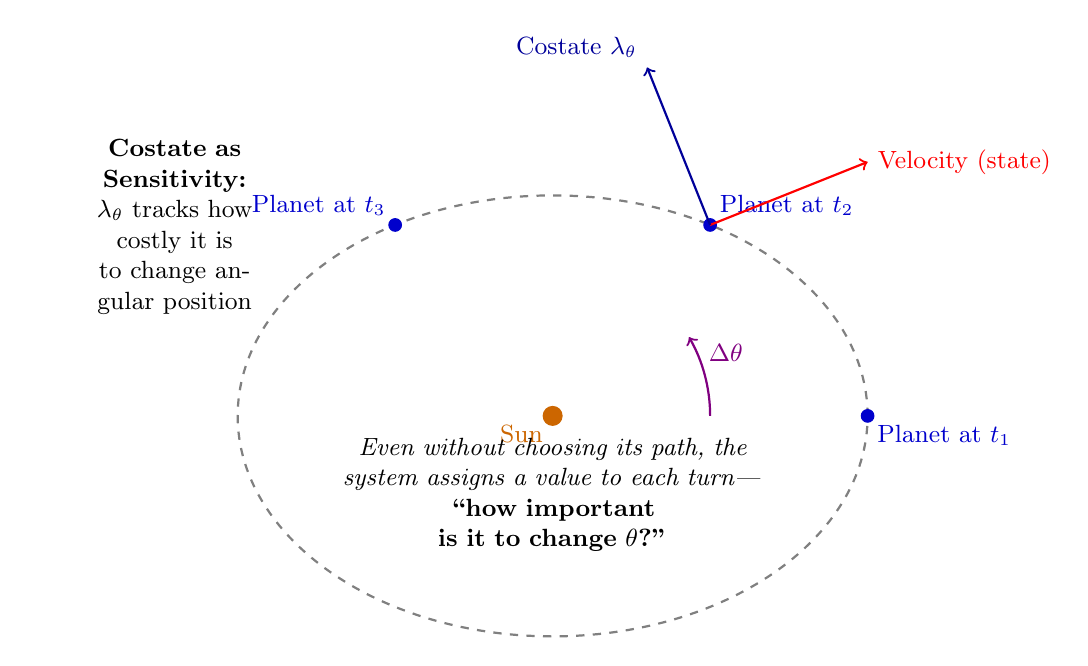
\begin{tikzpicture}[scale=4, every node/.style={font=\small}]
        % Sun
        \filldraw[orange!80!black] (0,0) circle (0.03) node[below left] {Sun};
    
        % Orbit path (ellipse for visual variation)
        \draw[gray, thick, dashed] (0,0) ellipse (1 and 0.7);
    
        % Planet positions
        \coordinate (P1) at (1,0);
        \coordinate (P2) at ({cos(60)},{0.7*sin(60)});
        \coordinate (P3) at ({cos(120)},{0.7*sin(120)});
        
        \filldraw[blue!80!black] (P1) circle (0.02) node[below right] {Planet at $t_1$};
        \filldraw[blue!80!black] (P2) circle (0.02) node[above right] {Planet at $t_2$};
        \filldraw[blue!80!black] (P3) circle (0.02) node[above left] {Planet at $t_3$};
    
        % Angular displacement arrows
        \draw[->, thick, violet] (0.5,0) arc (0:30:0.5);
        \node[violet] at (0.55,0.2) {$\Delta \theta$};
    
        % Tangent arrows
        \draw[->, red, thick] (P2) -- ++(0.5,0.2) node[right] {Velocity (state)};
        \draw[->, blue!60!black, thick] (P2) -- ++(-0.2,0.5) node[above left] {Costate $\lambda_\theta$};
    
        % Label costate interpretation
        \node[align=center, text width=3.5cm] at (-1.2,0.6) {
            \textbf{Costate as Sensitivity:}\\
            $\lambda_\theta$ tracks how costly it is \\
            to change angular position
        };
    
        % Message box
        \node[align=center, text width=5.5cm] at (0.0,-0.25) {
            \textit{Even without choosing its path, the system assigns a value to each turn—} \\
            \textbf{“how important is it to change $\theta$?”}
        };
    \end{tikzpicture}
    \caption{The orbit reinterpreted: not just a geometric path, but a structured solution to an implicit optimization. The costate $\lambda_\theta$ acts as a dynamic weight on angular change, assigning “value” to different directions of motion.}
\end{figure}


\begin{figure}[H]
    \centering
    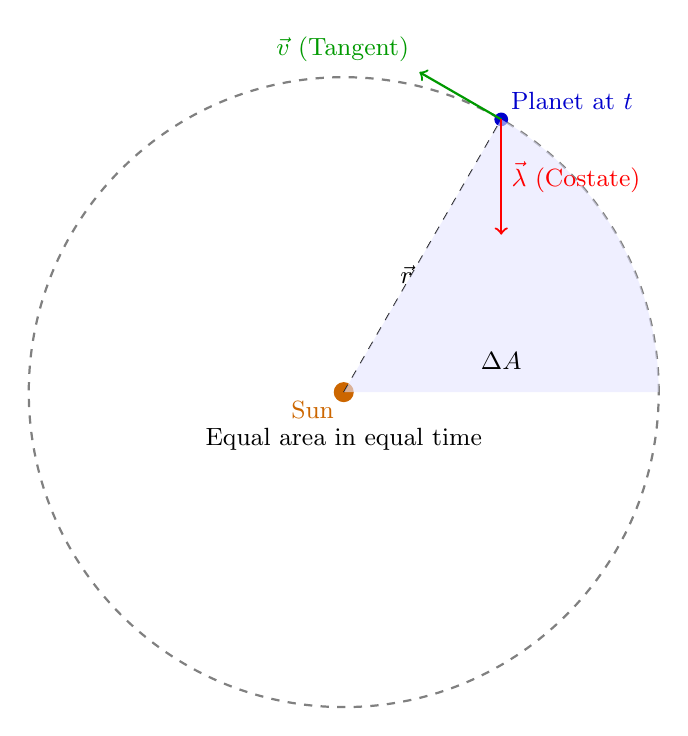
\begin{tikzpicture}[scale=4, every node/.style={font=\small}]
        % Sun
        \filldraw[orange!80!black] (0,0) circle (0.03) node[below left] {Sun};
    
        % Orbit path
        \draw[gray, thick, dashed] (0,0) circle (1);
    
        % Planet position
        \coordinate (P) at ({cos(60)},{sin(60)});
        \filldraw[blue!80!black] (P) circle (0.02) node[above right] {Planet at $t$};
    
        % Radius vector
        \draw[dashed] (0,0) -- (P) node[midway, below left] {$\vec{r}$};
    
        % Swept area
        \fill[blue!10, opacity=0.6] (0,0) -- (1,0) arc (0:60:1) -- cycle;
        \node at (0.5,0.1) {$\Delta A$};
    
        % Velocity vector (tangent)
        \draw[->, thick, green!60!black] (P) -- ++({-sin(60)*0.3},{cos(60)*0.3}) node[above left] {$\vec{v}$ (Tangent)};
    
        % Costate vector (radial)
        \draw[->, thick, red] (P) -- (0.5,0.5) node[midway, right] {$\vec{\lambda}$ (Costate)};
    
        % Label: Equal areas
        \node at (0,-0.15) {Equal area in equal time};
    
    \end{tikzpicture}
    \caption{Proper control-theoretic interpretation: the velocity vector is tangent to the orbit, and the costate vector (representing the sensitivity to angular change) points radially inward, reflecting the value of changing angle $\theta$.}
\end{figure}



\begin{figure}[H]
    \centering
    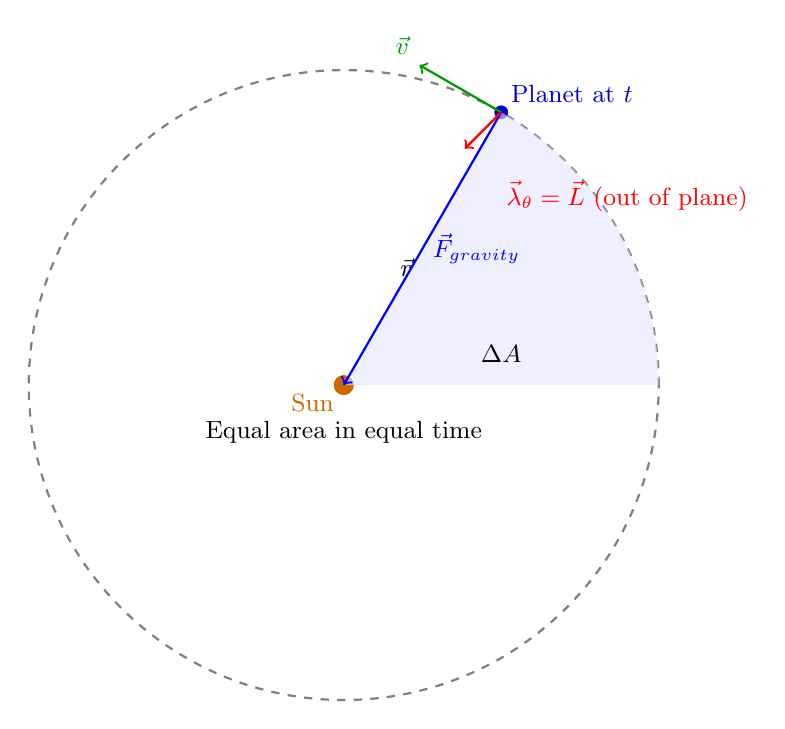
\begin{tikzpicture}[scale=4, every node/.style={font=\small}]
        % Sun
        \filldraw[orange!80!black] (0,0) circle (0.03) node[below left] {Sun};
    
        % Orbit path
        \draw[gray, thick, dashed] (0,0) circle (1);
    
        % Planet position
        \coordinate (P) at ({cos(60)},{sin(60)});
        \filldraw[blue!80!black] (P) circle (0.02) node[above right] {Planet at $t$};
    
        % Radius vector
        \draw[dashed] (0,0) -- (P) node[midway, below left] {$\vec{r}$};
    
        % Swept area
        \fill[blue!10, opacity=0.6] (0,0) -- (1,0) arc (0:60:1) -- cycle;
        \node at (0.5,0.1) {$\Delta A$};
    
        % Velocity vector (tangent to orbit)
        \draw[->, thick, green!60!black] (P) -- ++({-sin(60)*0.3},{cos(60)*0.3}) node[above left] {$\vec{v}$};
    
        % Force vector (toward Sun)
        \draw[->, thick, blue] (P) -- (0,0) node[midway, right] {\textcolor{blue}{$\vec{F}_\text{gravity}$}};
    
        % Costate / angular momentum vector (out of plane)
        \draw[->, thick, red] (P) -- ++(0,0,0.3);
        \node[red] at (0.9,0.6) {\textbf{\(\vec{\lambda}_\theta = \vec{L}\)} (out of plane)};
    
        % Label: Equal areas
        \node at (0,-0.15) {Equal area in equal time};
    
    \end{tikzpicture}
    \caption{In optimal control terms, the velocity is tangent to the orbit, the gravitational force points inward, and the costate associated with angular displacement corresponds to angular momentum — a vector normal to the orbital plane.}
\end{figure}


\textbf{Interpretation:} In the framework of optimal control theory, particularly Pontryagin’s Maximum Principle, we assign a \emph{costate} variable to each state variable. For a system governed by angular motion, the costate associated with angular displacement $\theta$ turns out to be angular momentum.

But it’s crucial to get the directions right.

\begin{itemize}
  \item The \textbf{velocity vector} $\vec{v}$ is always \textbf{tangent to the orbit}, representing the planet’s instantaneous motion.
  \item The \textbf{gravitational force} $\vec{F}_{\text{gravity}}$ pulls \textbf{radially inward} toward the Sun—this is the central force responsible for the curved path.
  \item The \textbf{costate} $\lambda_\theta$, though formally a scalar in Pontryagin’s equations, corresponds geometrically to \textbf{angular momentum}, which is a \textbf{vector perpendicular to the orbital plane}—pointing \textbf{out of the page} for counterclockwise orbits.
\end{itemize}

In this sense, the costate $\lambda_\theta$ can be interpreted as a kind of \emph{dynamic price tag} for changing the angle $\theta$. Its value represents how sensitive the system’s performance is to a small change in that direction. And just like angular momentum in classical mechanics, this “price” stays constant when there’s no torque—serving as a constraint that guides the entire motion.

The result is a powerful reinterpretation: Kepler’s equal-area law isn’t just a geometric curiosity—it’s a reflection of the constancy of this invisible “cost vector” that encodes the structure of the orbit.


